\subsection{任务二：Cipherfour 算法六轮最优差分与线性路线搜索}


\subsubsection{实验步骤}

\paragraph{（1）算法建模与平台配置}

本任务利用密码分析学课程实验平台，对 Cipherfour 算法分别进行六轮最优差分路线搜索与最优线性路线搜索。实验首先需要根据算法的轮函数结构编写平台配置文件，并通过平台提供的组件描述各轮之间的传播关系。因此，在正式配置算法之前，先对平台的变量命名规则及组件功能进行分析。

根据课程提供的使用指南，平台使用 \texttt{node\_r\_l\_j} 的形式命名状态变量，其中 $r$ 表示轮编号，$l$ 表示层编号，$j$ 表示该层中的变量位置。以课件中的 PRESENT 算法为例，每轮可以划分为 S 盒输入、S 盒输出、比特拆分及置换输出四个状态层，各层之间通过相应组件建立连接，具体结构如下图所示。

\begin{figure}[H]
    \centering
    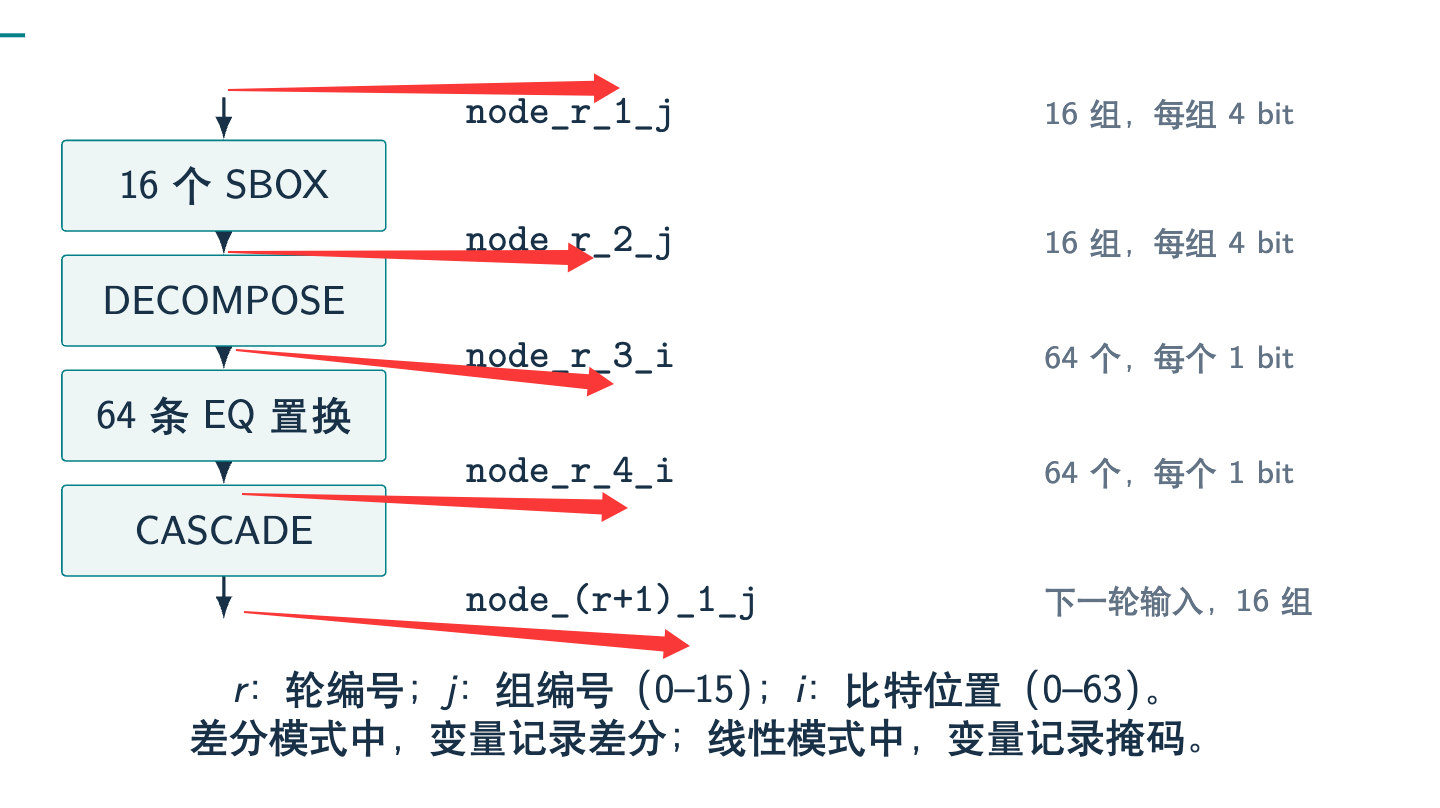
\includegraphics[width=0.95\textwidth]
    {figures/node.png}
\end{figure}

具体而言，第一层记录进入 S 盒之前的状态，第二层记录经过 S 盒替换后的输出状态。随后，通过 \texttt{DECOMPOSE} 组件将 S 盒输出拆分为单比特变量，形成第三层状态，以便对各个比特进行独立的置换操作。第三层与第四层之间通过 \texttt{EQ} 组件建立比特位置对应关系，完成置换后，再由 \texttt{CASCADE} 组件将单比特状态重新组合为下一轮 S 盒的输入。

在差分分析中，同一密钥下的轮密钥异或不会改变差分值，即
\[
(x\oplus k)\oplus(x'\oplus k)
=x\oplus x'.
\]
对于线性分析，固定轮密钥异或仅影响线性相关度的符号，不改变其绝对值。因此，在本次差分概率和线性相关度绝对值的路线搜索中，可以省略轮密钥异或组件，重点描述 S 盒替换及轮间比特置换。

在平台配置文件中，首先通过 \texttt{PARAMETERS} 定义算法使用的 S 盒参数，再利用 \texttt{SBOX}、\texttt{DECOMPOSE}、\texttt{EQ} 和 \texttt{CASCADE} 等组件描述各轮操作。课程提供的 PRESENT 配置示例已经展示了上述组件的组织方式，因此本实验以该示例为基础，根据 Cipherfour 的实际结构调整状态位宽、S 盒数量以及轮间连接关系。

\begin{figure}[H]
    \centering
    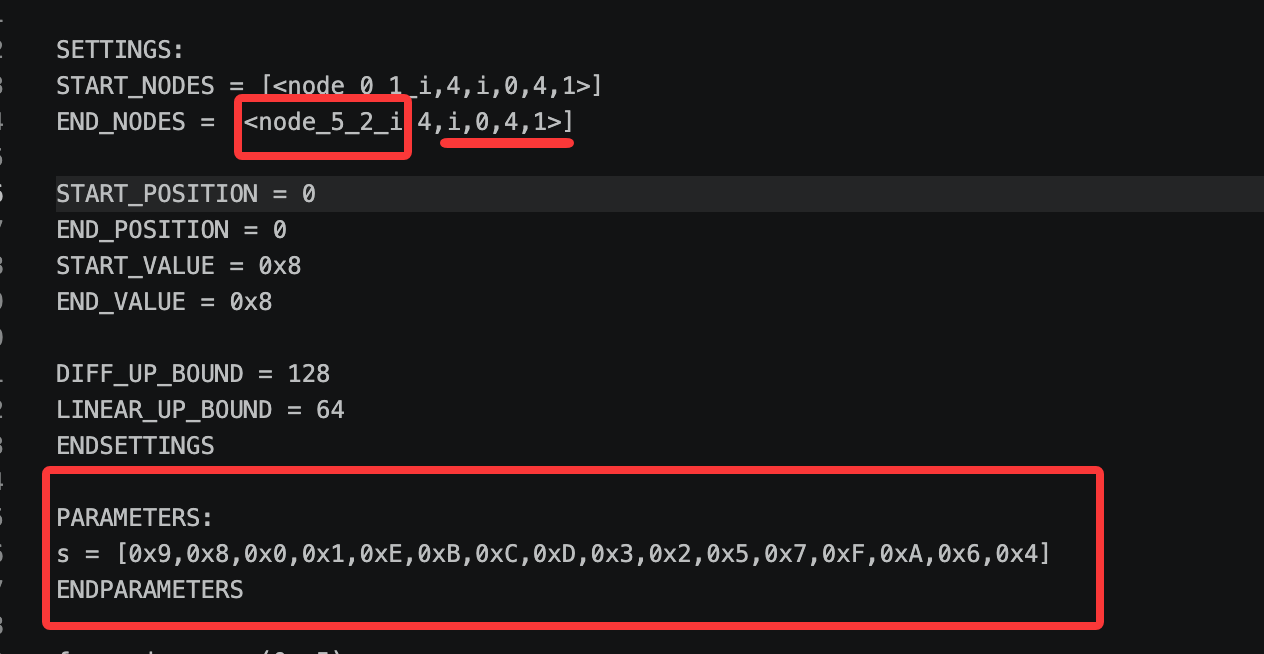
\includegraphics[width=0.95\textwidth]
    {figures/diff.png}
\end{figure}

与 PRESENT 算法的 $64$ bit 分组和 $16$ 个并行 S 盒不同，Cipherfour 的分组长度为 $16$ bit，每轮由 $4$ 个并行的 $4$ bit S 盒组成。因此，配置文件中需要将每轮 S 盒的循环次数调整为 $4$，并使用实验题目指定的 S 盒参数。Cipherfour 的轮函数结构如下图所示。

\begin{figure}[H]
    \centering
    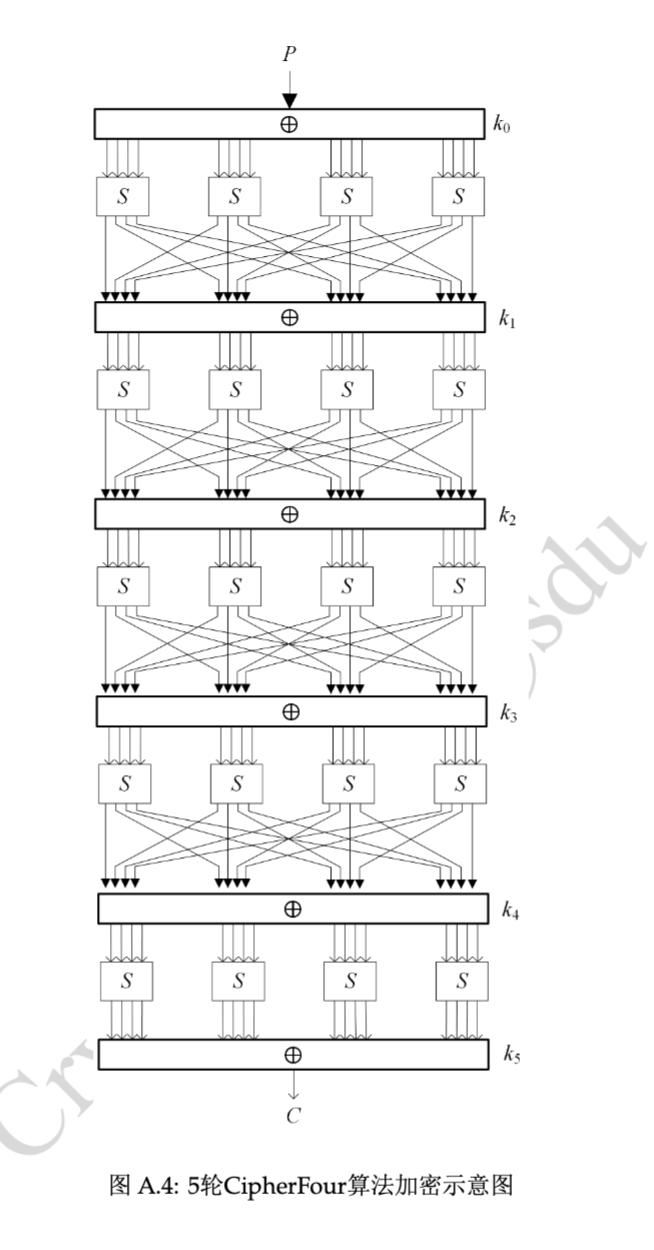
\includegraphics[width=0.3\textwidth]
    {figures/cipherfour.png}
\end{figure}

此外，本次使用的 Cipherfour 结构在最后一轮 S 盒替换后不再执行 P 置换，因此六轮模型中的前五轮需要描述 S 盒替换与轮间置换，而最后一轮只需保留 S 盒替换操作。由于平台的轮编号从 $0$ 开始，第六轮对应 $r=5$，其 S 盒输出位于第二层，因此模型的终止状态设置为
\[
\boxed{\texttt{node\_5\_2\_i}}.
\]

对于搜索参数，\texttt{DIFF\_UP\_BOUND} 和 \texttt{LINEAR\_UP\_BOUND} 分别用于设置差分分析与线性分析的初始搜索权重上界。本实验分别采用 $128$ 和 $64$ 作为初始上界，并通过平台的任务类型选择相应的搜索目标。两类分析使用相同的算法结构，但平台会根据所选任务采用不同的 S 盒传播约束及优化指标。

\begin{figure}[H]
    \centering
    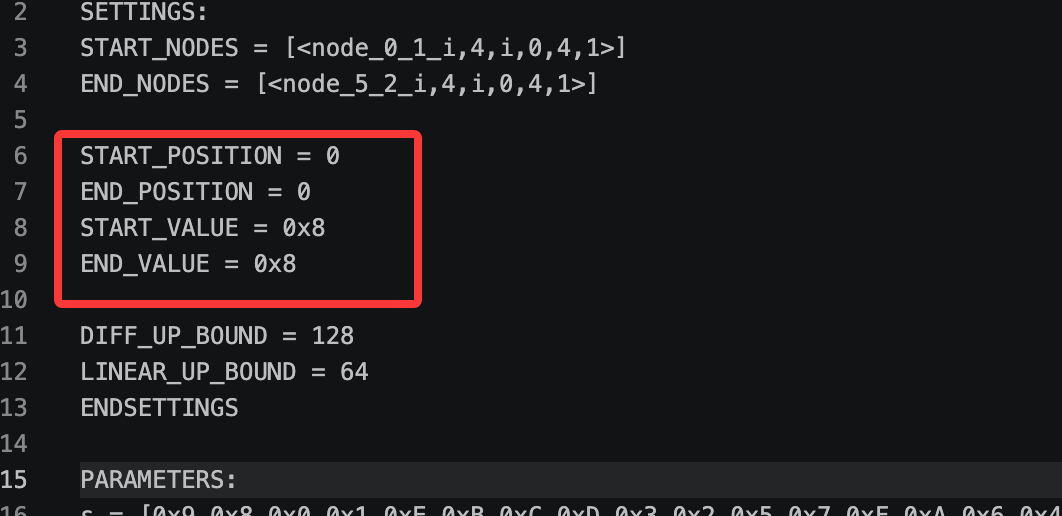
\includegraphics[width=0.95\textwidth]
    {figures/start.png}
\end{figure}

配置文件还包含 \texttt{START\_POSITION}、\texttt{END\_POSITION}、\texttt{START\_VALUE} 和 \texttt{END\_VALUE} 等边界参数。本次实验沿用课件中的示例设置，最终通过平台输出的路线及搜索结果进行核验。需要注意，这些参数是否实际参与搜索约束取决于平台所采用的具体任务模式，不能仅根据其配置值判断最终路线的起止状态是否受到限制。

\paragraph{（2）提交任务与调试}

完成算法配置后，将配置文件保存为 UTF-8 编码的文本文件，并上传至密码分析学课程实验平台。首先选择“概率最优差分路线”任务，对 Cipherfour 进行六轮差分路线搜索；随后保留相同的算法配置，将任务类型切换为“相关度最优线性路线”，完成对应的线性分析。

在首次提交差分任务时，平台显示任务失败，但未提供具体错误日志，因此无法直接确定问题来源。随后重新检查配置文件中的组件语法、循环范围、变量编号及轮间连接关系，并对部分配置进行调整。修改后，差分搜索成功运行；在此基础上继续提交线性搜索任务，也顺利获得了对应的分析结果。

本次实验最终完成了两项搜索任务，平台申请记录如图~\ref{fig:cipherfour-platform} 所示。

\begin{figure}[htbp]
    \centering
    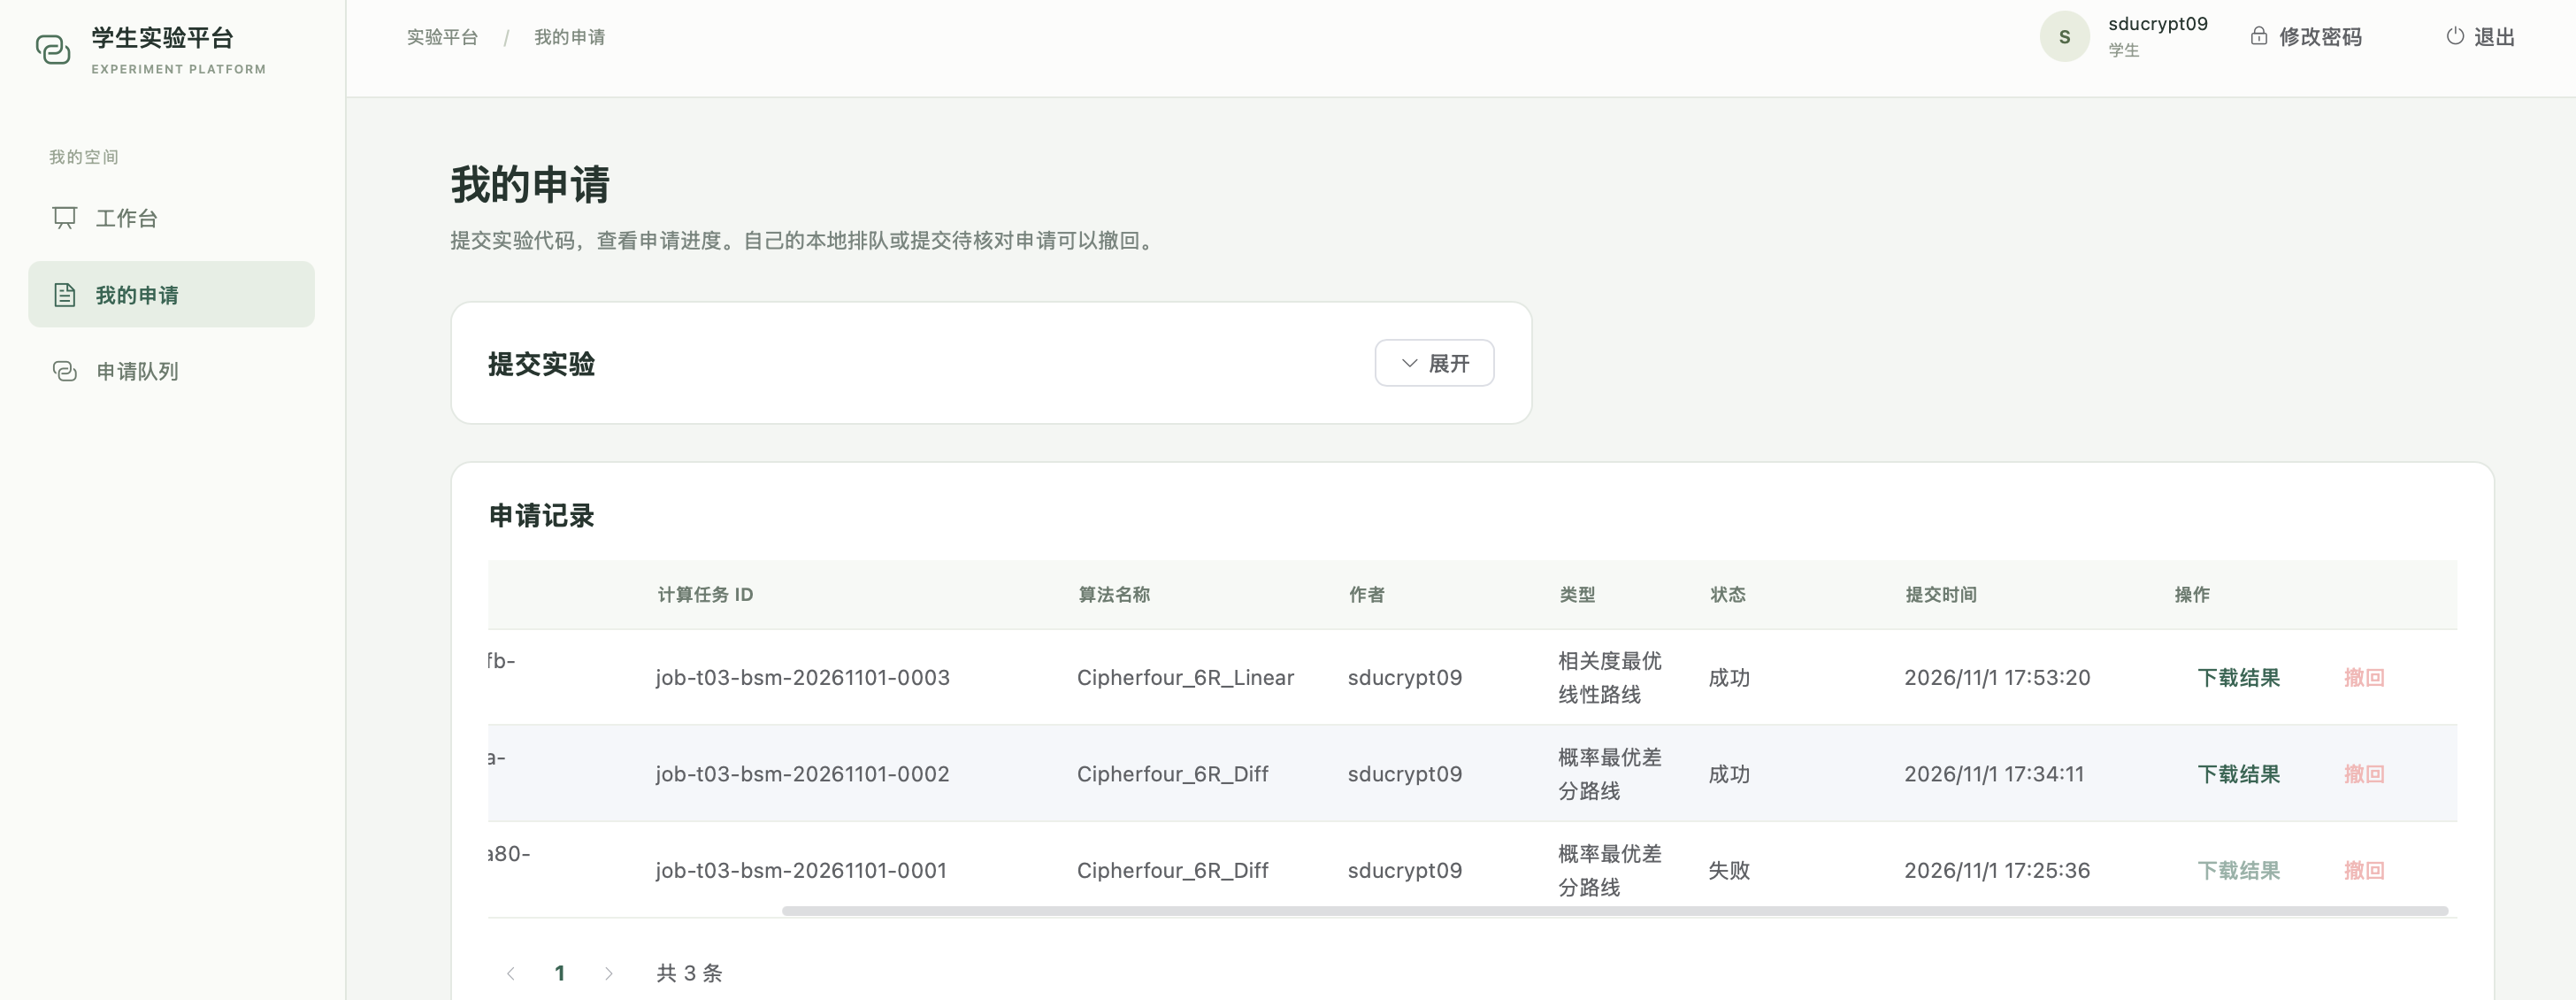
\includegraphics[width=0.95\textwidth]
    {figures/proof_of_the_platform.png}
    \caption{Cipherfour 差分与线性路线搜索任务的提交及运行结果}
    \label{fig:cipherfour-platform}
\end{figure}

\paragraph{（3）搜索结果提取与理论验证}

平台运行结束后，分别下载差分分析和线性分析对应的 \texttt{.rpt} 与 \texttt{.cvc} 文件。其中，\texttt{.rpt} 文件主要记录搜索迭代过程、求解状态、各轮输入输出差分或线性掩码，以及相应的概率或相关度指标；\texttt{.cvc} 文件则保存平台生成的约束求解模型，可用于进一步检查传播约束及权重表示方式。

根据差分搜索报告，平台首先在配置文件给定的初始权重上界 $128$ 下寻找可行路线。在首次成功搜索中，平台找到了一条概率为 $2^{-26}$ 的六轮差分路线，其对应的搜索日志如下图所示。

\begin{figure}[H]
    \centering
    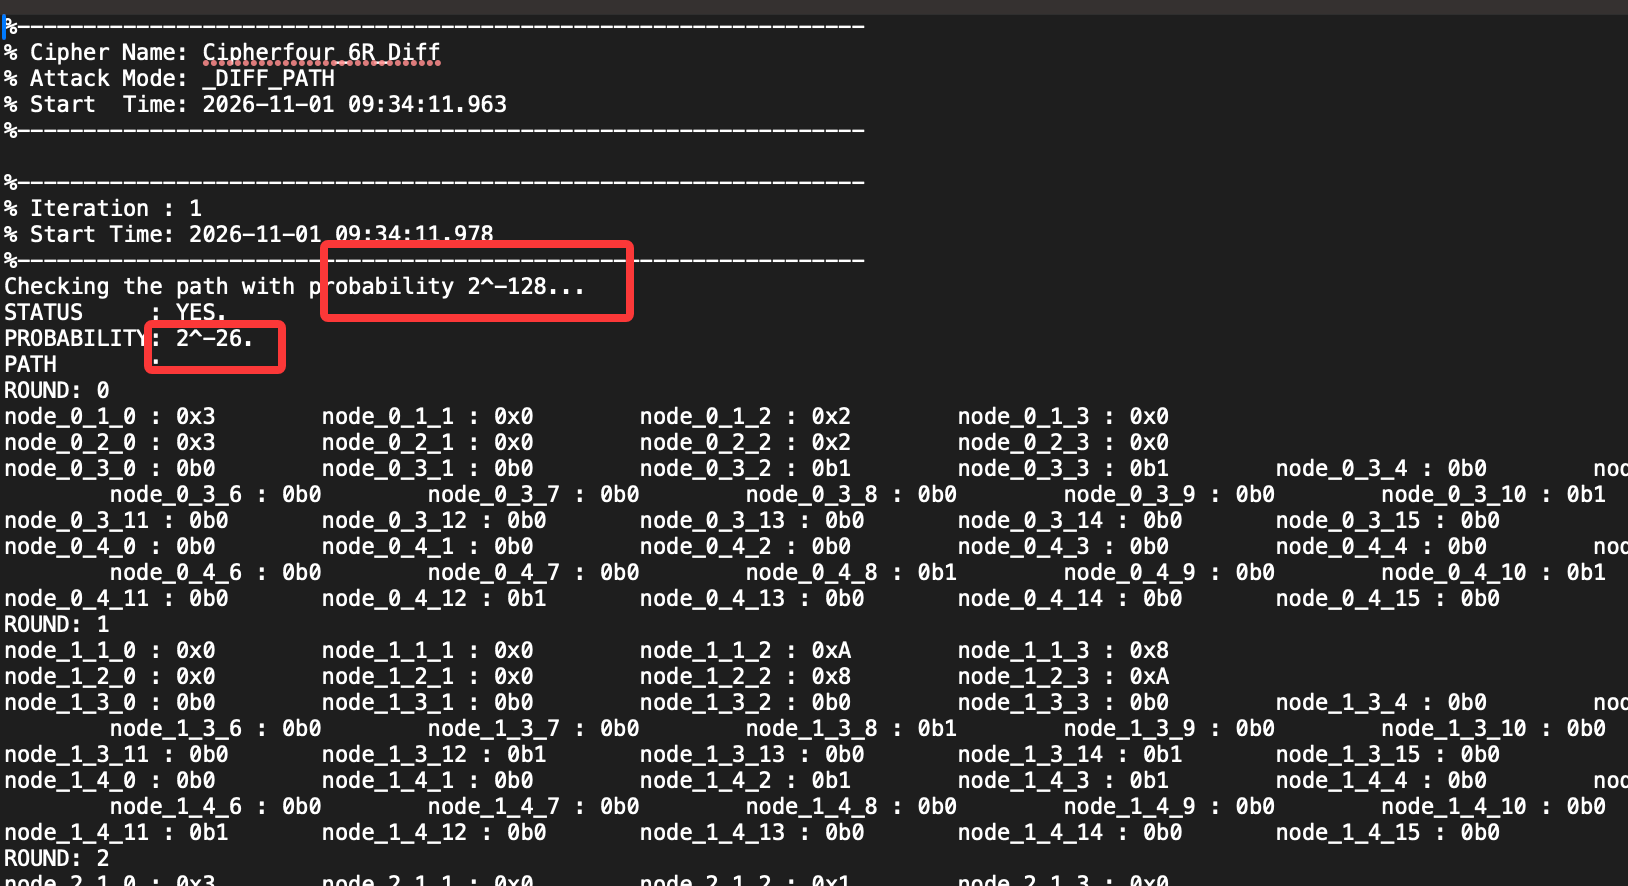
\includegraphics[width=0.95\textwidth]
    {figures/diff1.png}
\end{figure}

在获得可行路线后，平台进一步收紧搜索条件，将下一次搜索的概率阈值调整为 $2^{-25}$，继续寻找具有更高传播概率的路线。通过不断迭代，平台逐步提高候选路线的概率要求，直至无法找到满足更严格约束的路线，从而确定当前搜索模型下的最优差分权重。下一次迭代的运行情况如下图所示。

\begin{figure}[H]
    \centering
    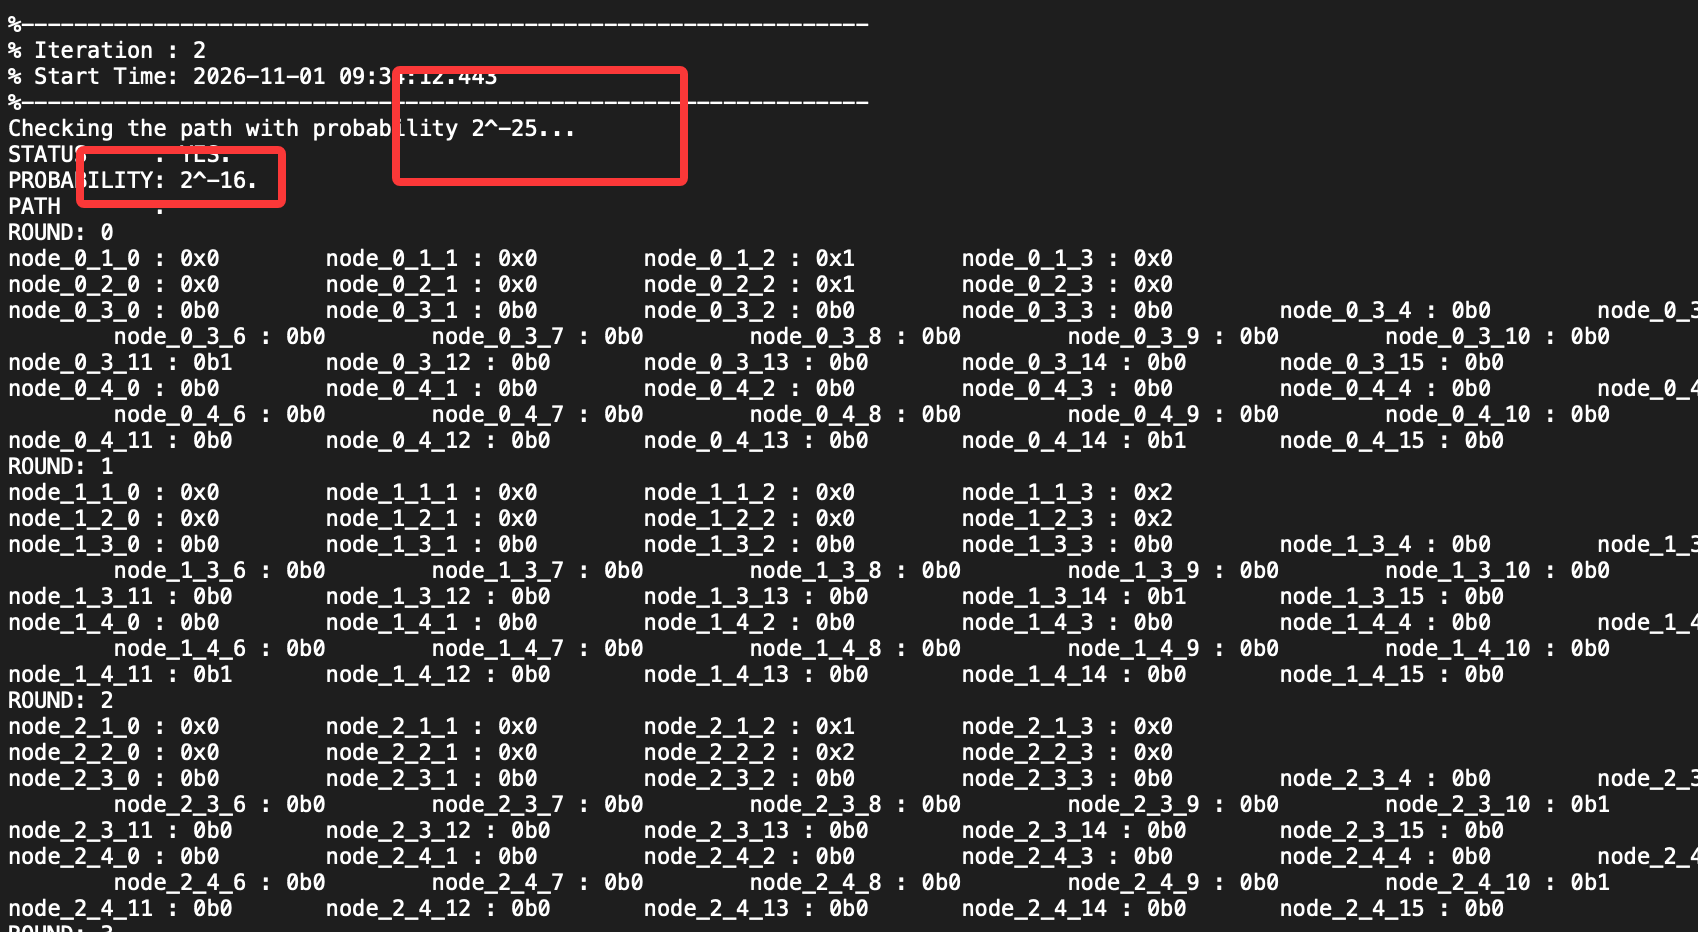
\includegraphics[width=0.95\textwidth]
    {figures/diff2.png}
\end{figure}

除搜索报告外，平台还生成了对应的 \texttt{.cvc} 约束文件。从文件内容可以观察到，平台将各轮状态变量及传播关系转化为位向量约束，并采用 STP/CVC 风格的语法组织相关表达式。其基本思想与任务一中使用 Gurobi 建立的约束模型具有相似性，即通过数学约束限定合法传播，再根据权重条件判断是否存在满足要求的路线。相关约束文件内容如下图所示。

\begin{figure}[H]
    \centering
    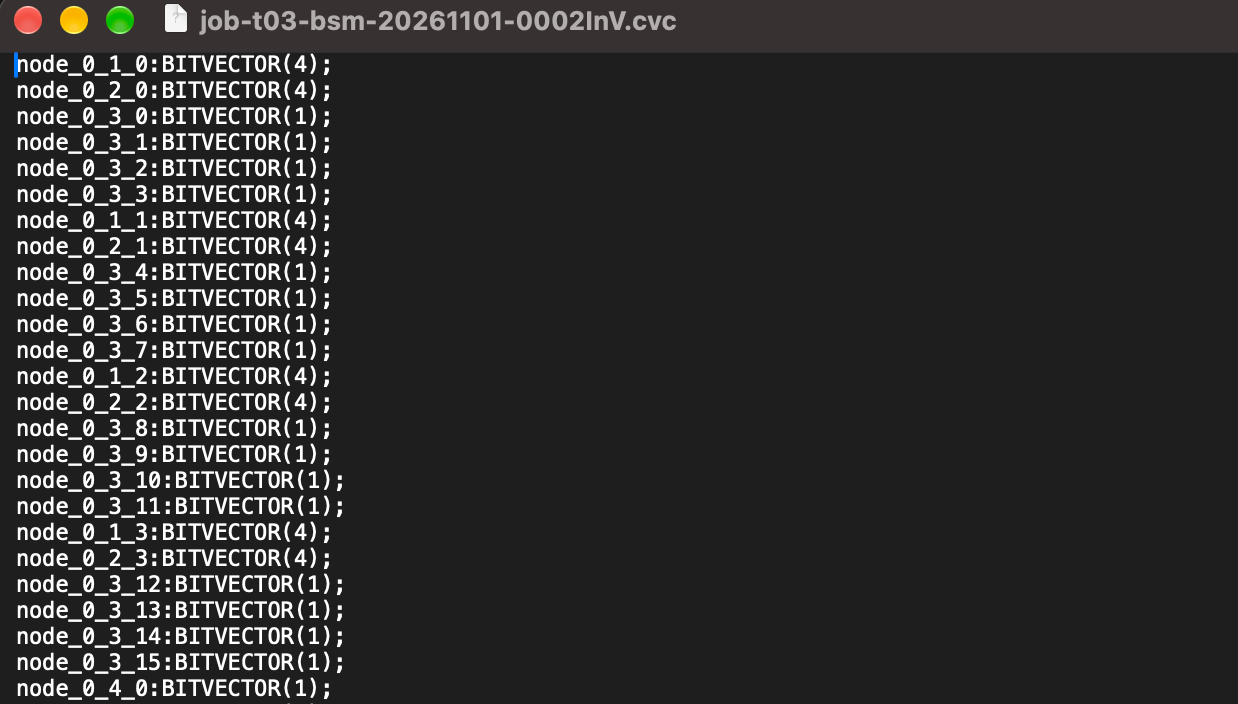
\includegraphics[width=0.95\textwidth]
    {figures/cvc.png}
\end{figure}

需要说明的是，虽然 \texttt{.cvc} 文件采用了与 STP 兼容的约束表示方式，但仅根据文件语法尚不能完全确定平台内部的具体求解器实现。因此，本实验主要将其用于分析平台生成的传播约束和权重编码方式，而不直接据此判断平台的完整求解流程。

在理论验证阶段，首先从 \texttt{.rpt} 文件中提取各轮输入输出差分及线性掩码，再分别利用任务一计算得到的 DDT 和 LAT 检查 S 盒局部传播的合法性与对应概率或相关度。同时，根据轮间比特置换关系检查相邻两轮状态是否正确连接，最后计算整条路线的概率或相关度，并将理论结果与平台输出进行比较，以验证搜索路线的准确性。



\subsubsection{实验结果及分析}

\paragraph{（1）六轮最优差分路线搜索}

差分分析任务的名称为
\texttt{Cipherfour\_6R\_Diff}。

平台采用逐步收紧概率下界的方式进行搜索。在第 $9$ 次迭代中，平台找到概率为 $2^{-6}$ 的可行差分路线；第 $10$ 次迭代进一步尝试搜索概率不低于 $2^{-5}$ 的路线，但求解结果为不可行。

对应的关键运行结果如下：
\begin{verbatim}
Iteration : 9
Checking the path with probability 2^-6...
STATUS     : YES.
PROBABILITY: 2^-6.

Iteration : 10
Checking the path with probability 2^-5...
STATUS     : No.
\end{verbatim}

由此可知，在当前六轮差分搜索模型下，最优差分路线的权重为
\[
W_D=6
\]
对应的差分路线概率为
\[
P_{\mathrm{trail}}=2^{-6}=\frac{1}{64}
\]

从第 $9$ 次迭代的输出中提取六轮差分路线，如表~\ref{tab:cipherfour-diff-path} 所示。

\begin{table}[htbp]
\centering
\caption{Cipherfour 六轮最优差分路线}
\label{tab:cipherfour-diff-path}
\begin{tabular}{c|c|c|c}
\hline
轮数 & 输入差分 & 输出差分 & 轮传播概率 \\
\hline
1 & \texttt{0x0001} & \texttt{0x0001} & $2^{-1}$ \\
2 & \texttt{0x0001} & \texttt{0x0001} & $2^{-1}$ \\
3 & \texttt{0x0001} & \texttt{0x0001} & $2^{-1}$ \\
4 & \texttt{0x0001} & \texttt{0x0001} & $2^{-1}$ \\
5 & \texttt{0x0001} & \texttt{0x0001} & $2^{-1}$ \\
6 & \texttt{0x0001} & \texttt{0x0001} & $2^{-1}$ \\
\hline
\end{tabular}
\end{table}
\begin{figure}[H]
    \centering
    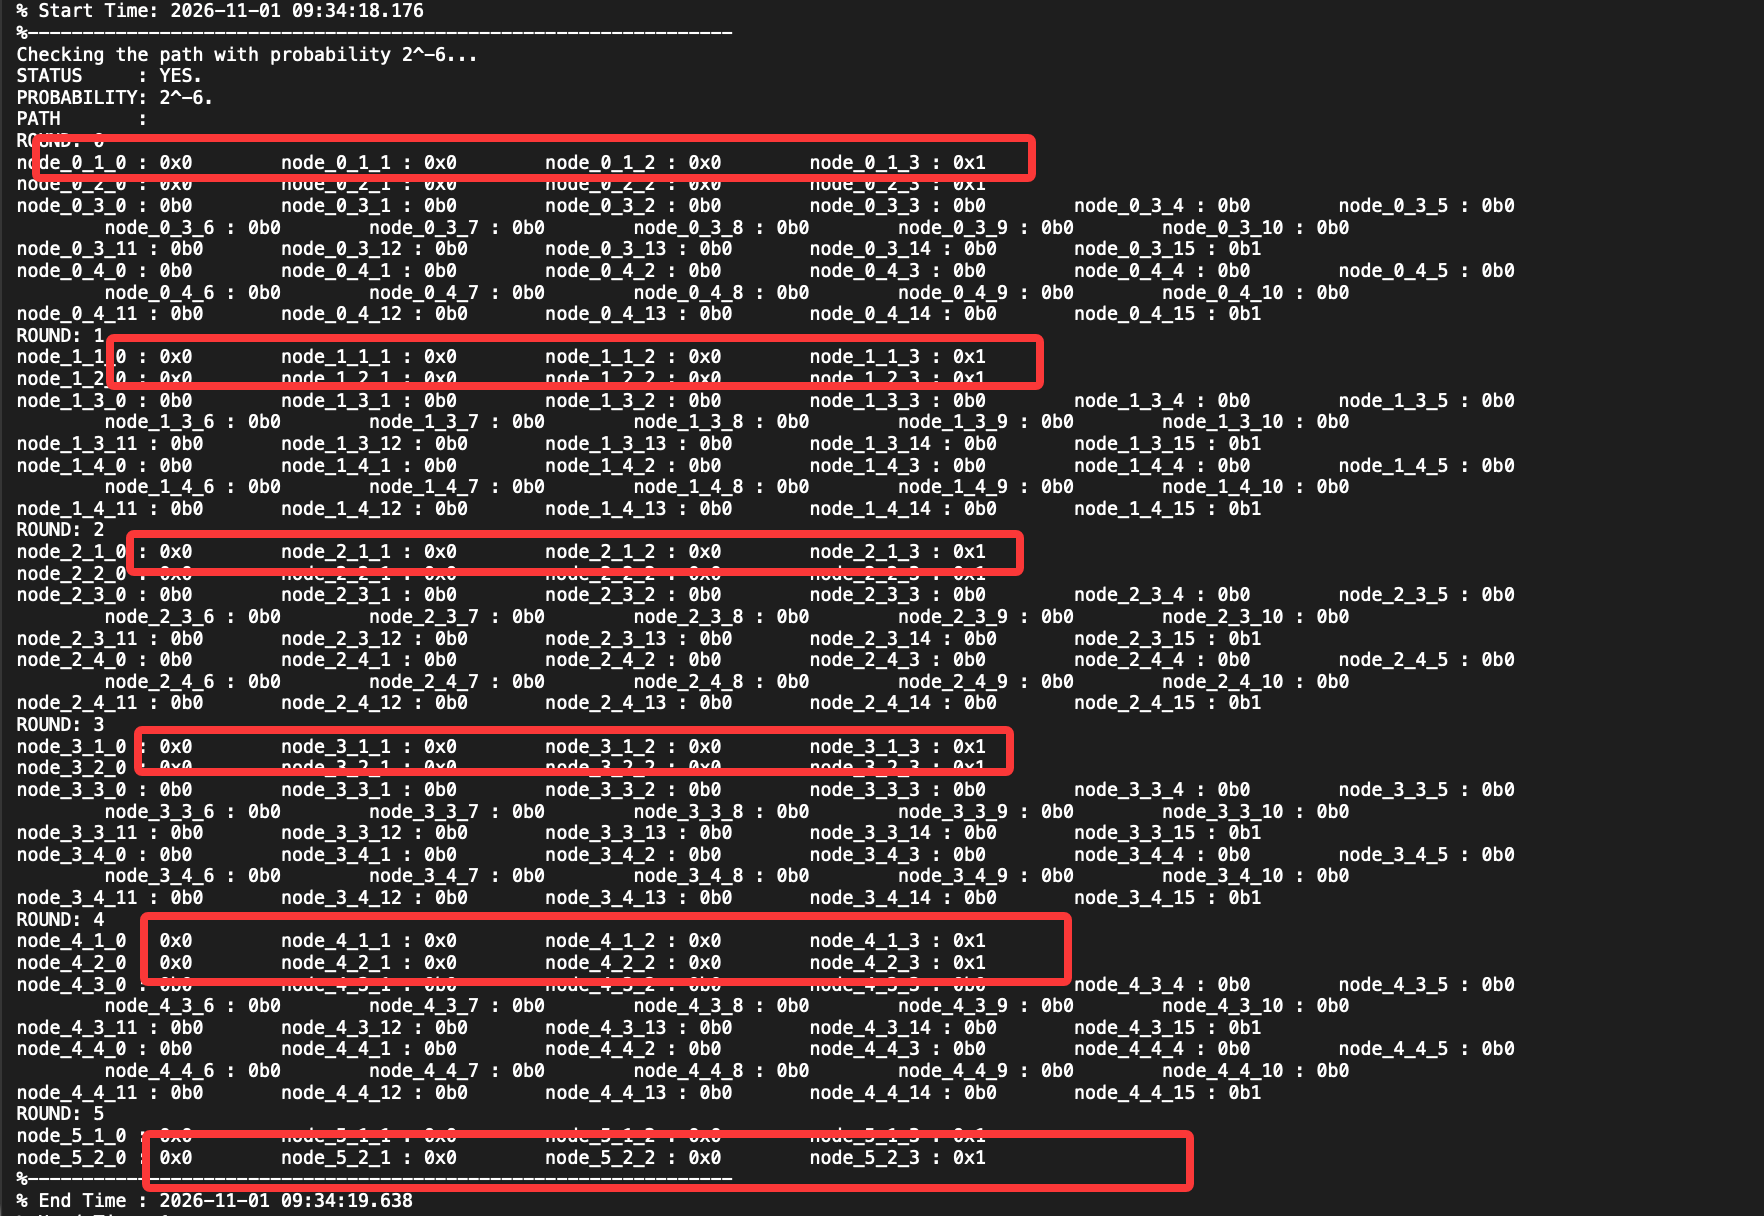
\includegraphics[width=0.8\textwidth]
    {figures/diff_res.png}
\end{figure}
可以发现，该路线的六轮输入输出差分均为 \texttt{0x0001}。每轮只有最低四比特对应的 S 盒处于活跃状态，其余三个 S 盒的输入输出差分均为 $0$。

根据任务一计算得到的 DDT，有
\[
\operatorname{DDT}[1][1]=8,
\qquad
\operatorname{DDT}[0][0]=16.
\]

因此，活跃 S 盒的差分传播概率为
\[
\Pr(1\rightarrow1)
=\frac{\operatorname{DDT}[1][1]}{16}
=\frac{8}{16}
=\frac12.
\]

对于其他三个非活跃 S 盒，有
\[
\Pr(0\rightarrow0)=1.
\]

因此，每轮四个 S 盒的联合传播概率为
\[
P_r=1\times1\times1\times\frac12
=\frac12.
\]

同时，由于该路线的非零差分位位于整个状态的最低位，在所采用的置换中有
\[
\pi(15)=15,
\]
因此该差分位经过置换后仍保持在原位置，可以在下一轮继续进行相同的传播。

综合六轮的传播概率，根据差分路线的概率乘积模型，有
\[
P_{\mathrm{trail}}=\prod_{r=1}^{6}P_r=\left(\frac12\right)^6=2^{-6}
\]

因此，理论计算结果与平台报告的差分路线概率完全一致。

结合第 $10$ 次迭代中更高概率阈值下无可行路线的结果，可以确认平台在当前差分模型下找到了最优六轮差分路线。

\paragraph{（2）六轮最优线性路线搜索}

线性分析任务的名称为
\texttt{Cipherfour\_6R\_Linear}。

与差分分析类似，平台逐步收紧相关度对应的权重上界。

在第 $9$ 次迭代中，平台找到内部权重为 $3$ 的可行线性路线，并报告相关度指标为 $2^{-3}$；第 $10$ 次迭代继续搜索权重不超过 $2$ 的路线，结果为不可行。

关键运行结果如下：
\begin{verbatim}
Iteration : 9
Checking the path with correlation of 2^-3...
STATUS     : YES.
LINEAR CORELATION: 2^-3.

Iteration : 10
Checking the path with correlation of 2^-2...
STATUS     : No.
\end{verbatim}

因此，平台在其内部整数权重模型下得到的最优值为
\[
\widetilde{W}_L=3
\]

第 $9$ 次迭代输出的六轮线性路线如表~\ref{tab:cipherfour-linear-path} 所示。
\begin{figure}[H]
    \centering
    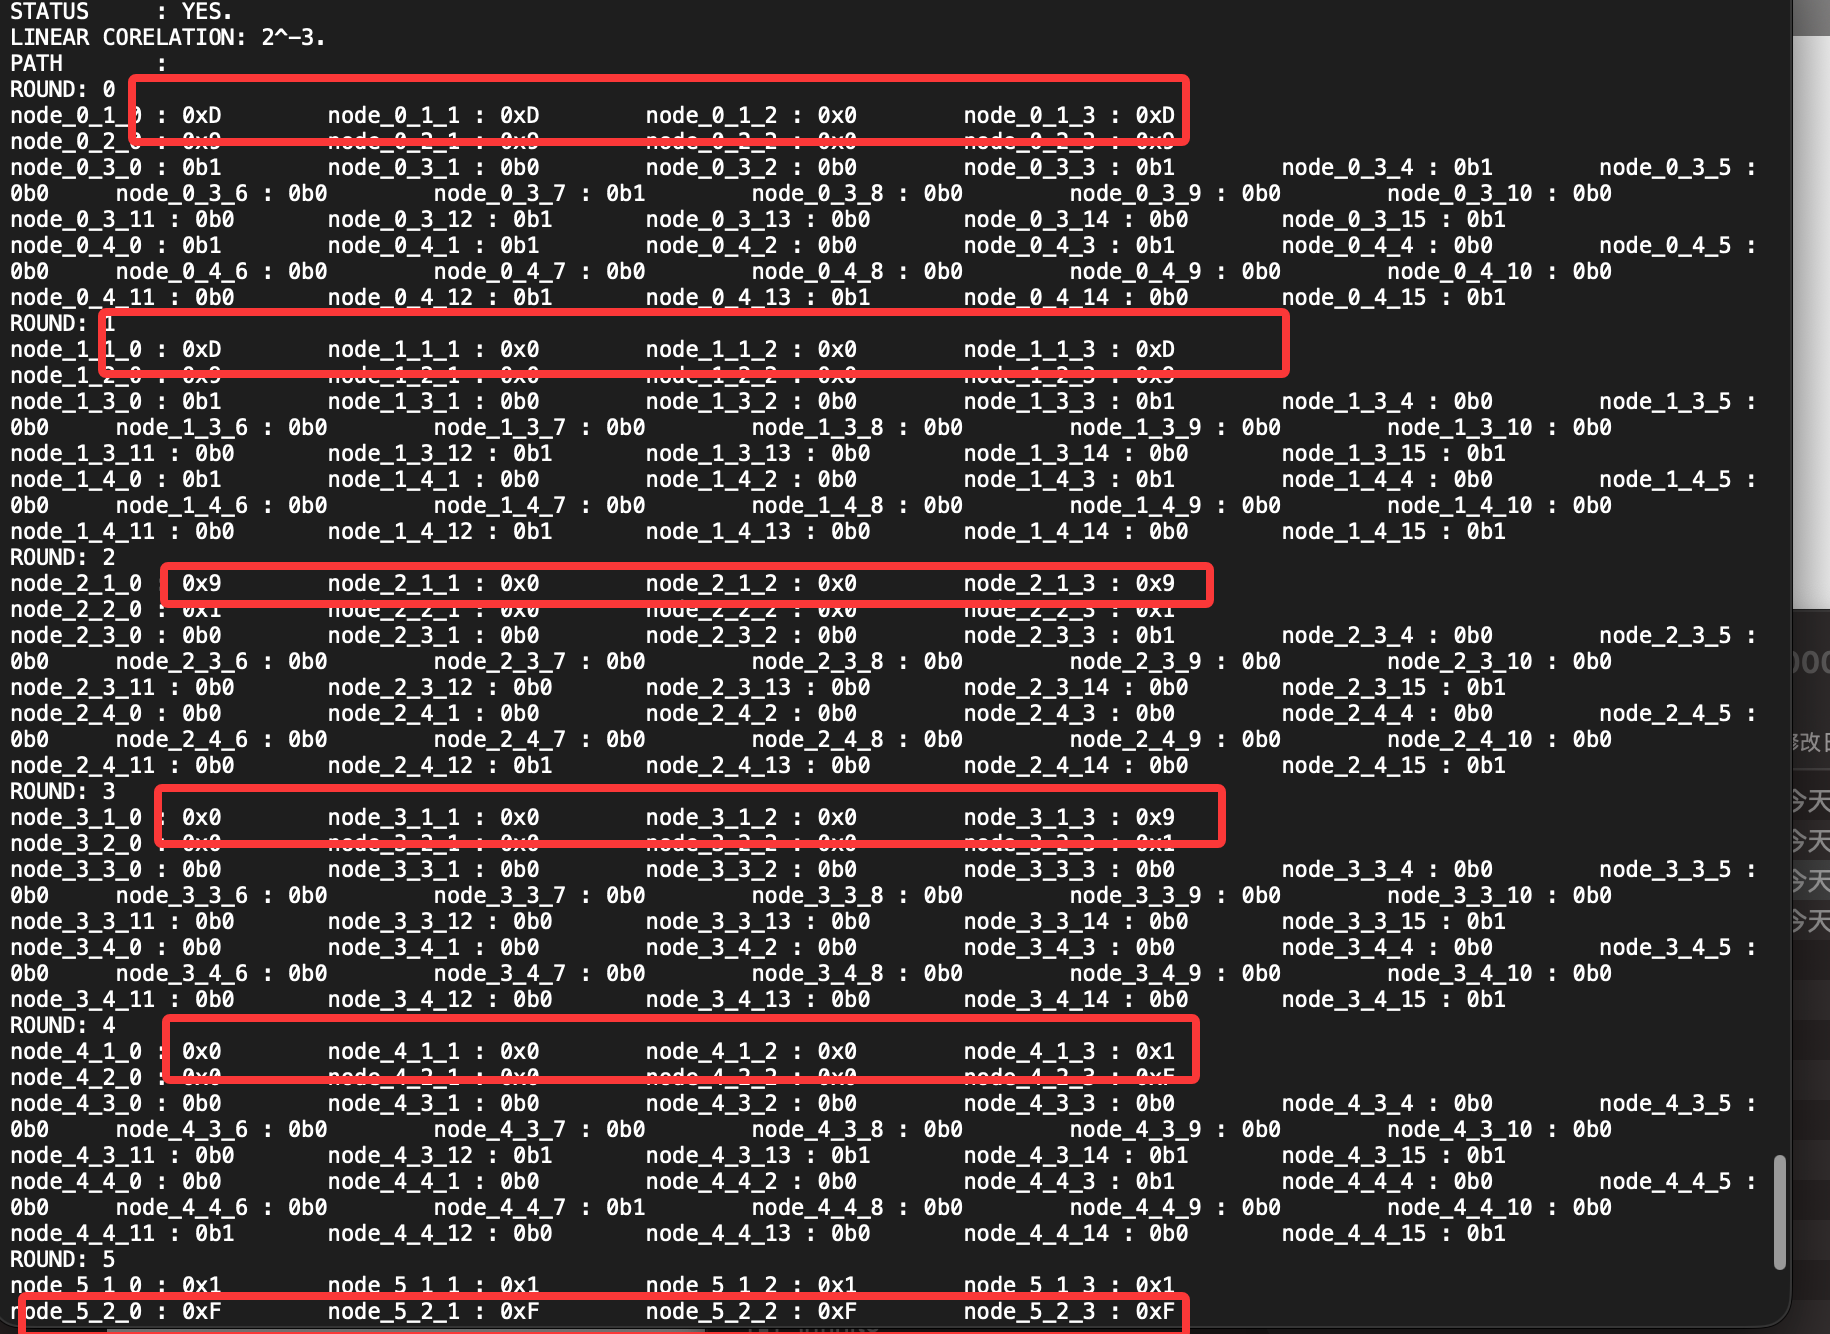
\includegraphics[width=0.8\textwidth]
    {figures/linear.png}
\end{figure}
\begin{table}[htbp]
\centering
\caption{Cipherfour 平台搜索得到的六轮线性路线}
\label{tab:cipherfour-linear-path}
\begin{tabular}{c|c|c|c}
\hline
轮数 & 输入掩码 & 输出掩码 & 精确轮相关度绝对值 \\
\hline
1 & \texttt{0xDD0D} & \texttt{0x9909}
  & $(3/4)^3$ \\
2 & \texttt{0xD00D} & \texttt{0x9009}
  & $(3/4)^2$ \\
3 & \texttt{0x9009} & \texttt{0x1001}
  & $(1/2)^2$ \\
4 & \texttt{0x0009} & \texttt{0x0001}
  & $1/2$ \\
5 & \texttt{0x0001} & \texttt{0x000F}
  & $3/4$ \\
6 & \texttt{0x1111} & \texttt{0xFFFF}
  & $(3/4)^4$ \\
\hline
\end{tabular}
\end{table}

为了验证上述路线，首先根据任务一的 LAT 计算各个 S 盒输入输出掩码对的相关度。

对于输入掩码 $\alpha$ 和输出掩码 $\beta$，定义 S 盒的 Walsh 相关和为
\[
W(\alpha,\beta)
=
\sum_{x\in\mathbb{F}_2^4}
(-1)^{\alpha\cdot x\oplus\beta\cdot S(x)}.
\]

其对应的相关度为
\[
C(\alpha,\beta)=\frac{W(\alpha,\beta)}{16}.
\]

若 LAT 使用偏差计数
$\operatorname{LAT}[\alpha][\beta]=N_0-8$
的定义，则有
\[
W(\alpha,\beta)
=2\operatorname{LAT}[\alpha][\beta].
\]

观察平台给出的线性路线，可以发现其中只涉及以下四种 S 盒局部传播：

\begin{table}[htbp]
\centering
\caption{线性路线所涉及的 S 盒局部相关度}
\label{tab:cipherfour-local-correlation}
\begin{tabular}{c|c|c|c}
\hline
输入掩码 & 输出掩码 & Walsh 值 & 相关度 \\
\hline
\texttt{0x0} & \texttt{0x0} & $16$ & $1$ \\
\texttt{0xD} & \texttt{0x9} & $12$ & $3/4$ \\
\texttt{0x9} & \texttt{0x1} & $8$ & $1/2$ \\
\texttt{0x1} & \texttt{0xF} & $12$ & $3/4$ \\
\hline
\end{tabular}
\end{table}

由表~\ref{tab:cipherfour-local-correlation} 可知，上述局部传播的相关度均不为零，因此均属于合法的线性掩码传播。

进一步检查相邻两轮的掩码关系，发现各轮 S 盒输出掩码经过比特置换后，均与下一轮 S 盒的输入掩码一致，说明该路线满足算法的轮间连接约束。

按照线性路线相关度的乘积公式，
\[
C_{\mathrm{trail}}
=
\prod_{r=1}^{6}\prod_{j=0}^{3}C_{r,j},
\]
其中 $C_{r,j}$ 表示第 $r$ 轮第 $j$ 个 S 盒的局部相关度。

对该路线中的局部传播进行统计，共有
$10$ 个相关度为 $3/4$ 的传播、
$3$ 个相关度为 $1/2$ 的传播，
其余 $11$ 个位置的相关度均为 $1$。

因此，
\[
\begin{aligned}
|C_{\mathrm{trail}}|
&=\left(\frac34\right)^{10}
  \left(\frac12\right)^3\\
&=\frac{59049}{8388608}\\
&\approx 0.00703919
\end{aligned}
\]

对应的精确线性权重为
\[
\begin{aligned}
W_L
&=-\log_2|C_{\mathrm{trail}}|\\
&\approx 7.1504
\end{aligned}
\]

需要注意的是，精确计算得到的线性权重与平台报告的整数权重 $3$ 并不相同。

为分析这一差异，进一步检查平台生成的 \texttt{.cvc} 文件中的 S 盒权重编码，发现平台对非零相关度使用的权重符合
\[
\widetilde{w}(\alpha,\beta)
=
\left\lfloor
-\log_2|C(\alpha,\beta)|
\right\rfloor.
\]

例如，对于相关度为 $3/4$ 的局部传播，
\[
-\log_2\frac34\approx0.415,
\]
经过向下取整后，平台将其编码为
\[
\widetilde{w}=0.
\]

而对于相关度为 $1/2$ 的局部传播，则有
\[
\widetilde{w}
=-\log_2\frac12
=1.
\]

因此，该路线在平台内部的总权重为
\[
\begin{aligned}
\widetilde{W}_L
&=10\times0+3\times1+11\times0\\
&=3
\end{aligned}
\]

这一结果与平台报告完全一致。

由此说明，平台报告的 $2^{-3}$ 是其整数化权重模型对应的搜索指标，而根据原始 LAT 计算得到的该路线精确相关度绝对值约为 $0.00703919$。

因此，平台成功找到了整数化权重模型下的最优线性路线，但该结果不能直接作为精确相关度全局最优性的证明。

\paragraph{（3）实验结果总结}

本次实验利用课程自动化分析平台，完成了 Cipherfour 算法的六轮差分路线和六轮线性路线搜索，并根据任务一计算得到的 DDT 和 LAT 对搜索结果进行了独立验证

两项搜索结果汇总如表~\ref{tab:cipherfour-summary} 所示。

\begin{table}[H]
\centering
\caption{Cipherfour 六轮差分与线性搜索结果汇总}
\label{tab:cipherfour-summary}
\begin{tabular}{c|c|c|c}
\hline
分析类型 & 平台最优权重 & 平台报告指标 & 精确验证结果 \\
\hline
差分分析 & $6$ & $2^{-6}$ & $2^{-6}$ \\
线性分析 & $3$ & $2^{-3}$ & $0.00703919$ \\
\hline
\end{tabular}
\end{table}